\documentclass[11pt,compress,t,notes=noshow, xcolor=table]{beamer}

\input{../../style/preamble_new}
\usepackage{tcolorbox}

% ToC
\AtBeginSection[]{
	\begin{frame}[noframenumbering, plain]
	\frametitle{Outline}
	\setcounter{tocdepth}{1}
	\tableofcontents[currentsection]
\end{frame}
}

\title{Deep Learning for NLP II}

\begin{document}

\titlemeta{
Retrieval-Augmented Generation (RAG)
}{}{
figure/rag-title.png
}{
\item Understand RAG pipelines
\item Overview of retrieval methods
\item Understand RAG evaluation
\item Practical considerations
}

% ------------------------------------------------------------------------------

\begin{frame}{Outline}
\tableofcontents
\end{frame}

% ==============================================================================
% MOTIVATION & CONTEXT
% ==============================================================================

\section{Motivation}

\begin{frame}{Motivation}

\vfill

\textbf{Motivation:}

\vspace{1em}

\begin{itemize}
    \item LLMs can do \textbf{amazing} things -- but they are prone to hallucinations
    \item Many schemes of types of hallucinations exist \citebutton{Huang et al. (2025) \cite{huang2025survey}}{https://dl.acm.org/doi/10.1145/3703155}
    \item Examples: 
        \begin{itemize}
            \item \textit{Factuality hallucinations} contradicting facts
            \item \textit{Faithfulness hallucinations} lacking logical consistence
        \end{itemize}
    \item Real-world examples:
        \begin{itemize}
            \item Lawyers cited fake ChatGPT cases \citebutton{Reuters (2023)}{https://www.reuters.com/legal/new-york-lawyers-sanctioned-using-fake-chatgpt-cases-legal-brief-2023-06-22/}
            \item Air Canada chatbot hallucinated refund policy\\
								  $\rightarrow$ lost lawsuit \citebutton{CBC (2024)}{https://www.cbc.ca/news/canada/british-columbia/air-canada-chatbot-lawsuit-1.7116416}
        \end{itemize}
\end{itemize}

\vspace{1em}

\textbf{Idea of RAG:} Provide relevant external knowledge at inference time

\vfill

\end{frame}

% ------------------------------------------------------------------------------

\begin{frame}{The Original RAG Paper}

\vfill

\textbf{Setup:} Combine a \textit{parametric} memory (seq2seq generator) with a \textit{non-parametric} memory (dense document index) \citebutton{Lewis et al. (2020) \cite{lewis2020retrieval}}{https://proceedings.neurips.cc/paper/2020/file/6b493230205f780e1bc26945df7481e5-Paper.pdf}

\begin{center}
	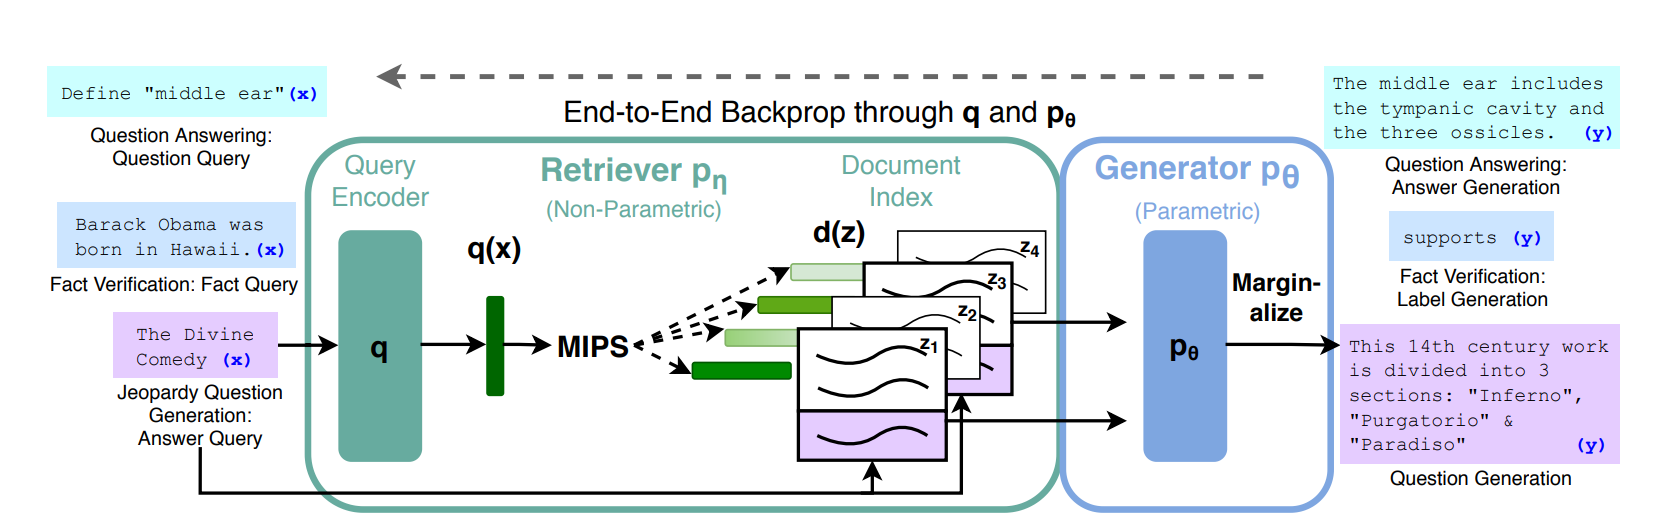
\includegraphics[width=10cm]{figure/rag.png}\\
	\citebutton{Source: \cite{lewis2020retrieval}}{https://proceedings.neurips.cc/paper/2020/file/6b493230205f780e1bc26945df7481e5-Paper.pdf}
\end{center}

\begin{center}
\small
\begin{tabular}{ll}
\toprule
\textbf{Component} & \textbf{Choice} \\
\midrule
Retrieval & Embedding-based (separate \texttt{BERT} models for $q$ and $d$) \\
Document index & 21M Wikipedia passages \\
Generator & \texttt{BART-large} (400M params) \\
Training & \textbf{End-to-end, no retrieval supervision} \\
\bottomrule
\end{tabular}
\end{center}

\vfill

\end{frame}

% ------------------------------------------------------------------------------

\begin{frame}{Retrieval-Augmented Generation}

\textbf{Core idea/design choices:}
\begin{itemize}
    \item Retrieve relevant documents ("`\textit{evidence}"'), then generate answers grounded in this evidence
    \item Use increasingly strong (and expensive) models at each stage
    \item Example of typical 2-stage retrieval (retriever + reranker)
\end{itemize}

\vspace{0.1cm}

\begin{center}
\begin{tikzpicture}[
    node distance=0.4cm,
    box/.style={rectangle, draw=black, thick, minimum height=0.7cm, minimum width=1.3cm, font=\footnotesize},
    data/.style={rectangle, rounded corners, fill=blue!10, minimum height=0.5cm, font=\scriptsize},
    arrow/.style={->, thick, >=stealth}
]
    \node[data] (query) {Query};
    \node[box, right=of query, fill=green!20] (retriever) {Retriever};
    \node[data, right=of retriever] (topk) {Top-k};
    \node[box, right=of topk, fill=orange!20] (reranker) {Reranker};
    \node[data, right=of reranker] (topn) {Top-n};
    \node[box, right=of topn, fill=purple!20] (generator) {Generator};
    \node[data, right=of generator] (answer) {Answer};
    \draw[arrow] (query) -- (retriever);
    \draw[arrow] (retriever) -- (topk);
    \draw[arrow] (topk) -- (reranker);
    \draw[arrow] (reranker) -- (topn);
    \draw[arrow] (topn) -- (generator);
    \draw[arrow] (generator) -- (answer);
\end{tikzpicture}
\end{center}

\vfill

\begin{center}
\footnotesize
\begin{tabular}{lll}
\toprule
\textbf{Component} & \textbf{Latency} & \textbf{What it optimizes} \\
\midrule
Retriever (sparse vs. dense) & 100-300ms & Recall (M $\rightarrow$ 100s) \\
Reranker & 100-2000ms & Precision (100s $\rightarrow$ 10s) \\
Generator (LLM) & 1000+ms & Quality \\
\bottomrule
\end{tabular}
\end{center}

\end{frame}

% ------------------------------------------------------------------------------

\begin{frame}{Document Chunking}

\vfill

\textbf{From Documents to Retrievable Units:} Prior to retrieval we need document \textbf{chunks}, i.e., \textit{meaningful semantic units}\\ 

\vspace{1em}

 \textbf{Why chunk?}
 \begin{itemize}
     \item Long documents (100+ pages) consume too much LLM context
     \item Enables more precise retrieval of relevant passages
 \end{itemize}

\vspace{1em}

 \textbf{Trade-offs:}
 \begin{center}
 \small
 \begin{tabular}{lll}
 \toprule
 \textbf{Size} & \textbf{Pros} & \textbf{Cons}  \\
 \midrule
 Smaller & Precise matching & Loses context  \\
 Larger & Preserves context & Adds noise  \\
 \bottomrule
 \end{tabular}
 \end{center}

 \vfill

\end{frame}

% ------------------------------------------------------------------------------

\begin{frame}{Document Chunking: Strategies (1)}

\vspace{0.5em}

\textbf{Fixed-size splitting} (baseline)
\begin{itemize}
    \item Split every $n$ tokens, optionally with overlap
    \item Fast, but may cut mid-sentence or mid-argument
\end{itemize}

\vspace{1em}

\textbf{Recursive splitting} \citebutton{LangChain docs}{https://docs.langchain.com/oss/python/integrations/splitters}
\begin{itemize}
    \item Try splitting on ``\texttt{\textbackslash n\textbackslash n}'' first, then ``\texttt{\textbackslash n}'', then spaces -- falling back to the next separator only if chunks are still too large
    \item Naturally respects paragraphs $>$ sentences $>$ words;\\
		Recommended in LangChain
\end{itemize}

\vspace{1em}

\textbf{Sentence-boundary-aware splitting}
\begin{itemize}
    \item Respect sentence boundaries\\(e.g.\ via spaCy / NLTK sentence segmentation)
    \item Chunks stay linguistically coherent; embeddings are more meaningful (compared to fixed-size splitting)
\end{itemize}

\end{frame}

% ------------------------------------------------------------------------------

\begin{frame}{Document Chunking: Strategies (2)}

\vspace{0.5em}

\textbf{Semantic chunking}
\begin{itemize}
    \item Embed consecutive sentences; insert a boundary wherever cosine similarity \textit{drops} (more than a predefined theshold)
    \item Groups sentences that talk about the same topic -- boundaries follow content, not word count
\end{itemize}

\vspace{0.6em}

\textbf{Parent-document retriever} \citebutton{LangChain docs}{https://python.langchain.com/docs/how_to/parent_document_retriever/}
\begin{itemize}
    \item Index \textit{small} child chunks for precise retrieval \ldots
    \item \ldots but return the \textit{larger} parent passage to the generator
    \item \textit{Best of both worlds:} 
			\begin{itemize}
				\item fine-grained matching
				\item sufficient context for generation
			\end{itemize}
\end{itemize}

\vfill

\end{frame}

% ==============================================================================
% RETRIEVAL METHODS
% ==============================================================================

\section{Retrieval Methods}

\begin{frame}{Retrieval Methods: Overview}

\vfill

\textbf{Three main pillars:}

\vfill

\begin{center}
\begin{tikzpicture}[
    node distance=2cm,
    method/.style={rectangle, draw, thick, minimum width=2.5cm, minimum height=1cm, font=\small, align=center}
]
    \node[method, fill=yellow!20] (bm25) {BM25\\\scriptsize(Sparse)};
    \node[method, fill=green!20, right=of bm25] (dense) {SBERT/DPR\\\scriptsize(Dense)};
    \node[method, fill=blue!20, right=of dense] (hybrid) {Combinations\\\scriptsize(Hybrid)};

    \node[below=0.4cm of bm25, font=\scriptsize, text=gray] {statistical};
    \node[below=0.4cm of dense, font=\scriptsize, text=gray] {text embedding};
    \node[below=0.4cm of hybrid, font=\scriptsize, text=gray] {merges rankings};
\end{tikzpicture}
\end{center}

\vfill

\textbf{Key insight:} \\
No single best method -- tradeoffs between speed, accuracy and interpretability

\vfill

\end{frame}

% ------------------------------------------------------------------------------

\begin{frame}{BM25: Best Match 25}

\vfill

\textbf{Representation:} BM25 represents documents as sparse vectors (one dimension per vocabulary term) \citebutton{Robertson \& Zaragoza (2009) \cite{robertson2009probabilistic}}{https://dl.acm.org/doi/10.1561/1500000019}

\vfill

\textbf{Three intuitions}:
\begin{enumerate}
    \item \textbf{Rare terms matter more} (IDF): ``transformer'' $>$ ``the''
    \item \textbf{Diminishing returns} (TF saturation):\\
					saying ``good'' 10$\times$ $\neq$ 10$\times$ more relevant
    \item \textbf{Length normalization}: longer docs not automatically better
\end{enumerate}

\vfill

\begin{tabular}{ll}
\toprule
\textbf{Strengths} & \textbf{Limitations} \\
\midrule
Fast implementation & Vocabulary mismatch (``car'' $\neq$ ``automobile'') \\
Interpretable & No semantic understanding \\
\bottomrule
\end{tabular}

\end{frame}

% ------------------------------------------------------------------------------

\begin{frame}{BM25: Best Match 25 -- Formula (1)}

\vspace{1em}

\textbf{Scoring function} (for query $Q = \{q_1,\dots,q_n\}$ and document $D$):

\[
\text{BM25}(D,Q) = \sum_{i=1}^{n} \underbrace{\text{IDF}(q_i)}_{\text{term weight}} \cdot \underbrace{\frac{f(q_i,D)\,(k_1+1)}{f(q_i,D) + k_1\!\left(1-b+b\,\tfrac{|D|}{\text{avgdl}}\right)}}_{\text{term frequency (saturated \& length-normalised)}}
\]

\vspace{0.5em}

\textbf{Component breakdown:}
\begin{itemize}
    \item $f(q_i,D)$: raw term frequency of $q_i$ in $D$
    \item $|D|$ / $\text{avgdl}$: document length relative to corpus average\\
          $\rightarrow$ prevents long documents from being favoured by chance
    \item $k_1 \in [1.2, 2.0]$: \textbf{TF saturation} -- controls how fast the TF contribution plateaus (e.g.\ $k_1{=}0$ $\Rightarrow$ pure IDF; $k_1{\to}\infty$ $\Rightarrow$ raw TF)
\end{itemize}

\vfill

\end{frame}

% ------------------------------------------------------------------------------

\begin{frame}{BM25: Best Match 25 -- Formula (2)}

\vspace{1em}

\textbf{Scoring function} (for query $Q = \{q_1,\dots,q_n\}$ and document $D$):

\[
\text{BM25}(D,Q) = \sum_{i=1}^{n} \underbrace{\text{IDF}(q_i)}_{\text{term weight}} \cdot \underbrace{\frac{f(q_i,D)\,(k_1+1)}{f(q_i,D) + k_1\!\left(1-b+b\,\tfrac{|D|}{\text{avgdl}}\right)}}_{\text{term frequency (saturated \& length-normalised)}}
\]

\vspace{0.5em}

\textbf{Component breakdown:}
\begin{itemize}
    \item $b \in [0,1]$: \textbf{length normalization strength}\\
          ($b{=}0$: no normalization, $b{=}1$: full normalization)
    \item $\text{IDF}(q_i) = \log\!\frac{N - n(q_i) + 0.5}{n(q_i) + 0.5}$: inverse document frequency\\
          ($N$ = corpus size, $n(q_i)$ = number of docs containing $q_i$)
\end{itemize}

\vfill

\textbf{Defaults:} $k_1 = 1.5$, $b = 0.75$ work well across many collections

\end{frame}

% ------------------------------------------------------------------------------

\begin{frame}{From Statistical to embedding-based (1)}

\vfill

\textbf{Remember:} Word embeddings (e.g., word2vec) give fixed vectors per word, but do not carry sentence-level meaning

\vspace{1em}

\textbf{Initial idea:} Use BERT to classify sentence similarity (\textbf{cross-encoder})
\begin{center}
\texttt{[CLS] sent A [SEP] sent B [SEP]} $\rightarrow$ BERT $\rightarrow$ \textit{similar / not similar}
\end{center}
\vspace{1em}
\begin{center}
	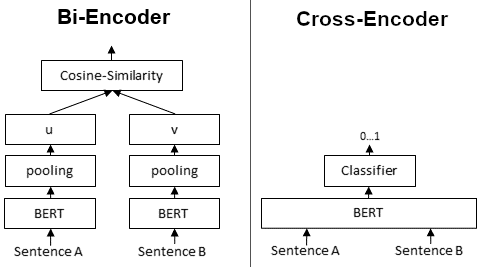
\includegraphics[width=3.5cm, clip, trim = 6.75cm 0 0 3cm]{figure/bi-vs-cross}\\
	\citebutton{Source: SBERT homepage}{https://www.sbert.net/examples/cross_encoder/applications/README.html}
\end{center}

\vfill

\end{frame}

% ------------------------------------------------------------------------------

\begin{frame}{From Statistical to embedding-based (2)}

\textbf{Problem:} Requires $O(n^2)$ comparisons!
\begin{itemize}
    \item Finding most similar pair in 10,000 sentences = 50M comparisons ($\sim$65 hours!) \citebutton{Reimers \& Gurevych (2019) \cite{reimers-gurevych-2019-sentence}}{https://aclanthology.org/D19-1410/}
    \item Not suitable for retrieval at scale
\end{itemize}

\vspace{1em}

\textbf{Idea:} Learn fixed-size sentence embeddings that can be pre-computed

\begin{center}
\begin{tikzpicture}[
    node distance=0.5cm,
    box/.style={rectangle, draw, thick, minimum height=0.5cm, font=\small},
    data/.style={rectangle, rounded corners, fill=blue!10, font=\small},
    arrow/.style={->, thick, >=stealth}
]
    \node[data] (sent) {Sentence};
    \node[box, fill=green!20, right=of sent] (enc) {Encoder};
    \node[data, right=of enc] (vec) {768-dim vector};
    \node[box, fill=orange!20, right=of vec] (cos) {Cosine similarity};

    \draw[arrow] (sent) -- (enc);
    \draw[arrow] (enc) -- (vec);
    \draw[arrow] (vec) -- (cos);
\end{tikzpicture}
\end{center}

\begin{center}
	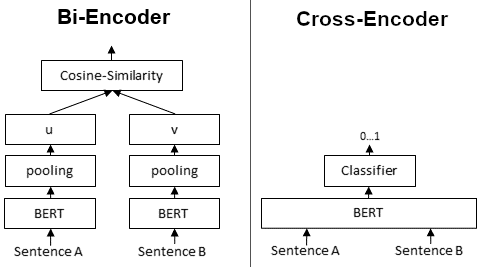
\includegraphics[width=6cm]{figure/bi-vs-cross}\\
	\citebutton{Source: SBERT homepage}{https://www.sbert.net/examples/cross_encoder/applications/README.html}
\end{center}

\vfill

\end{frame}

% ------------------------------------------------------------------------------

\begin{frame}{Sentence-BERT (SBERT)}
    \centering
    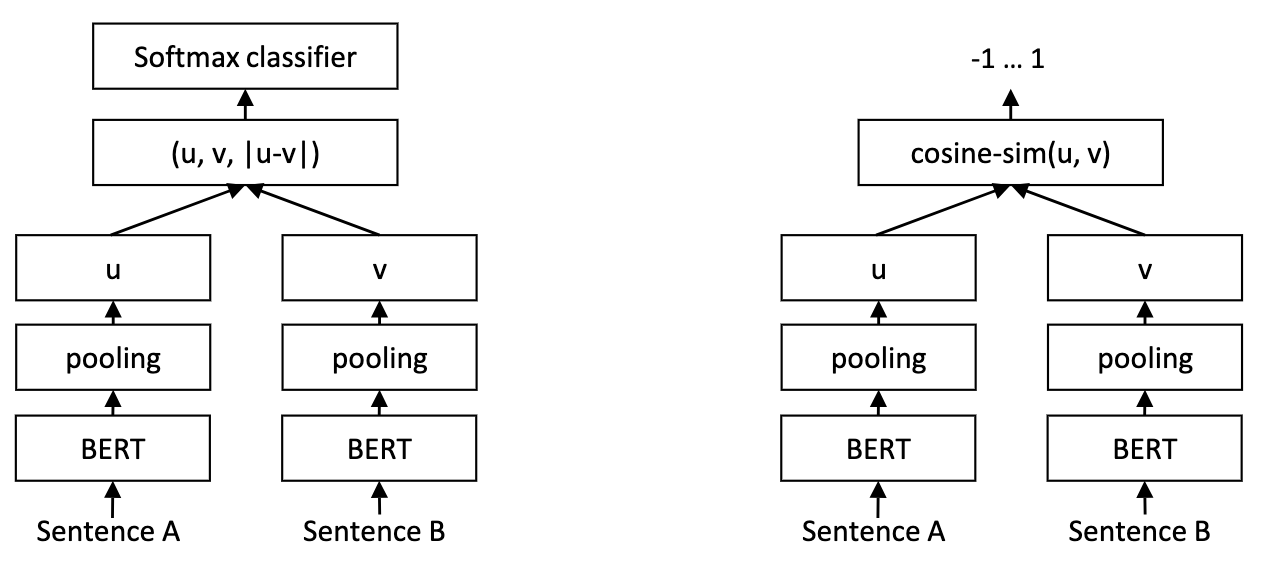
\includegraphics[width=9cm]{figure/sbert-architecture} \\
    {\hfill \scriptsize  Training (Shared weights) \hfill \hfill  Inference (Individual Encoders) \hfill }\\
		\citebutton{Source: \cite{reimers-gurevych-2019-sentence}}{https://aclanthology.org/D19-1410/}

    \vspace{1em}
    \textbf{Key Insight:} Shared BERT weights $\rightarrow$ comparable embedding space.

    \begin{itemize}
        \item \textbf{Symmetric search:} Find text that \textit{means the same thing}.
        \item \textbf{Training:} On NLI and Sentence Similarity Tasks
    \end{itemize}

    \textbf{Impact:} 10K comparisons reduced from 65 hours $\rightarrow$ \textbf{5 seconds}
    \vfill
\end{frame}

% ------------------------------------------------------------------------------

\begin{frame}{SBERT: Asymmetry Problem}

\vfill

\textbf{Problem:} SBERT is trained on general similarity, i.e., similar questions have similar embeddings and similar documents have similar embeddings.\\

$$questions \neq documents$$

\vspace{1em}

$\Rightarrow$ Retrieval might fail due to this asymmetry \\

\vspace{1em}

\textbf{Idea:} Train asymmetric embeddings, i.e. train whether an passage answers a question.\\

\vspace{1em}

\begin{center}
	\textit{Dense Passage Retrieval (DPR)} \citebutton{Karpukhin et al. (2020) \cite{karpukhin-etal-2020-dense}}{https://aclanthology.org/2020.emnlp-main.550/}
\end{center}

\vfill

\end{frame}

% ------------------------------------------------------------------------------

\begin{frame}{DPR (1): Overview}

\vfill

\begin{center}
\begin{tikzpicture}[
    node distance=0.4cm,
    box/.style={rectangle, draw=black, thick, minimum height=0.6cm, minimum width=1.8cm, font=\small},
    vec/.style={circle, draw=black, thick, minimum size=0.5cm, font=\small},
    arrow/.style={->, thick, >=stealth}
]
    % Query branch
    \node[box, fill=blue!10] (q) {Query};
    \node[box, fill=green!20, right=0.5cm of q] (eq) {$E_Q$ (BERT)};
    \node[vec, fill=blue!20, right=0.5cm of eq] (qvec) {$\mathbf{q}$};

    % Passage branch
    \node[box, fill=blue!10, below=0.8cm of q] (p) {Passage};
    \node[box, fill=orange!20, right=0.5cm of p] (ep) {$E_P$ (BERT)};
    \node[vec, fill=orange!20, right=0.5cm of ep] (pvec) {$\mathbf{p}$};

    % Dot product
    \node[right=0.8cm of qvec, yshift=-0.4cm] (dot) {$\mathbf{q} \cdot \mathbf{p}$};

    \draw[arrow] (q) -- (eq);
    \draw[arrow] (eq) -- (qvec);
    \draw[arrow] (p) -- (ep);
    \draw[arrow] (ep) -- (pvec);
    \draw[arrow] (qvec) -- (dot);
    \draw[arrow] (pvec) -- (dot);

    % Label
    \node[below=0.1cm of ep, font=\scriptsize, text=gray] {$E_Q \neq E_P$ (different params)};
\end{tikzpicture}
\end{center}

\vfill

\begin{center}
	
\small
\begin{tabular}{ll}
\toprule
\textbf{SBERT (Symmetric)} & \textbf{DPR (Asymmetric)} \\
\midrule
Same encoder (shared) & Different encoders ($E_Q \neq E_P$) \\
Trained on NLI/STS & Trained on QA pairs \\
\bottomrule
\end{tabular}
\normalsize

\end{center}

\end{frame}

\begin{frame}{DPR (2): Training \& Retrieval}

\vfill

\textbf{Training objective:} Maximize similarity of positive (question, passage) pairs and minimize it for negatives

\[
L = -\log \frac{e^{\mathbf{q}^{\top}\mathbf{p}^+}}{e^{\mathbf{q}^{\top}\mathbf{p}^+} + \sum_{j=1}^{m} e^{\mathbf{q}^{\top}\mathbf{p}^-_j}}
\]

\begin{itemize}
    \item $\mathbf{q} = E_Q(\text{[CLS]})$, $\mathbf{p} = E_P(\text{[CLS]})$ -- the [CLS] vectors of the respective BERT encoders
    \item Hard negatives: top BM25 passages that do \textit{not} answer the question $\rightarrow$ much more effective than random negatives
    \item In-batch negatives: other passages in the same mini-batch serve as cheap negatives
\end{itemize}

\vfill

\end{frame}

\begin{frame}{DPR (2): Training \& Retrieval}

\vfill

\textbf{Inference:}
\begin{enumerate}
    \item \textbf{Offline:} Encode all $M$ passages once with $E_P$ $\rightarrow$ store vectors
    \item \textbf{Online:} Encode query with $E_Q$ $\rightarrow$ retrieve top-$k$ by dot product
\end{enumerate}

\vfill

\textbf{Results:} 

\begin{center}
	DPR outperforms BM25 by $>$9\% EM on Natural Questions\\
\citebutton{Karpukhin et al. (2020) \cite{karpukhin-etal-2020-dense}}{https://aclanthology.org/2020.emnlp-main.550/}

\end{center}

\vfill

\end{frame}

% ------------------------------------------------------------------------------

\begin{frame}{Efficient Similarity Search}

\vfill

\textbf{Problem:} After encoding millions of passages, brute-force search is still slow.

\vfill

\textbf{FAISS} (Facebook AI Similarity Search): \citebutton{Douze et al. (2024) \cite{douze2024faiss}}{https://arxiv.org/abs/2401.08281}
\begin{itemize}
    \item Approximate Nearest Neighbor (ANN) search
    \item Trades exact results for massive speed gains
    \item DPR + FAISS searches 21M passages in \textbf{milliseconds}
\end{itemize}

\vfill

\begin{center}
\small
\begin{tabular}{llll}
\toprule
\textbf{Method} & \textbf{Speed} & \textbf{Recall} & \textbf{Memory} \\
\midrule
Flat (exact) & Slow & 100\% & High \\
IVF & Fast & $\sim$95\% & Medium \\
IVF+PQ & Very fast & $\sim$90\% & Low \\
\bottomrule
\end{tabular}
\end{center}

\vfill

\textbf{Key insight:} Similarity search is \textbf{solved infrastructure} -- use FAISS, Pinecone, Weaviate, \ldots

\vfill

\end{frame}

% ------------------------------------------------------------------------------

\begin{frame}{ColBERT: Late Interaction}

\vfill

\textbf{Problem:} Single-vector embeddings lose information \\
\textbf{Idea:} Preserve per-token representations

\begin{center}
    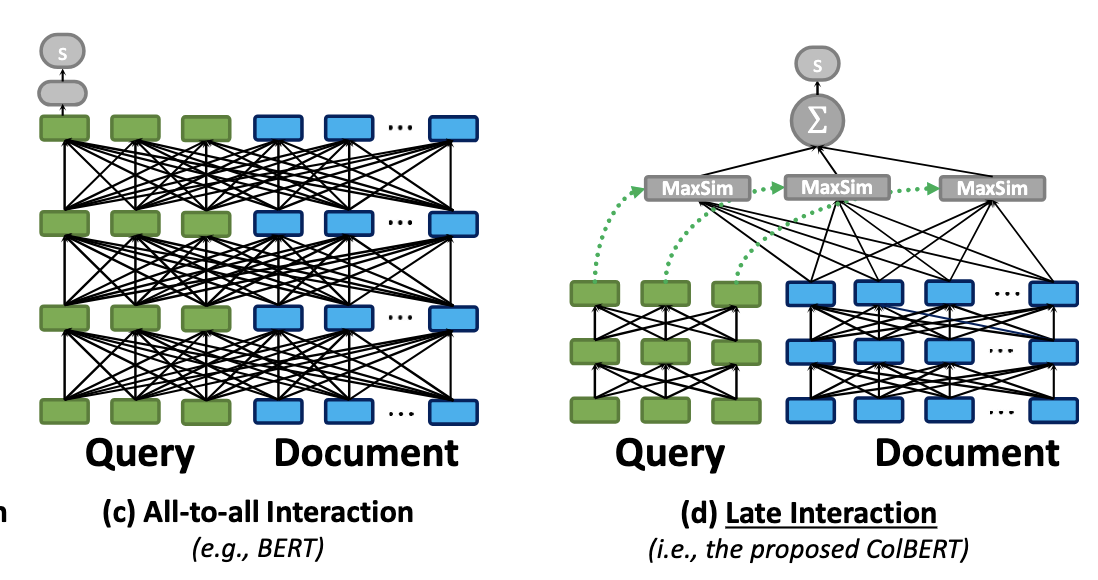
\includegraphics[width=0.7\textwidth,keepaspectratio]{figure/colbert-maxsim}\\
		{\scriptsize *\textbf{MaxSim score:} For each query token, find best-matching doc token, then sum scores}\\
		\citebutton{Source: \cite{colbert}}{https://dl.acm.org/doi/10.1145/3397271.3401075}
\end{center}
		
\vfill

\end{frame}

% ------------------------------------------------------------------------------

\begin{frame}{ColBERT: Late Interaction}

\vfill

\textbf{Comparison to cross-encoders:}

\begin{center}
\scriptsize
\begin{tabular}{lll}
\toprule
& \textbf{Cross-Encoder} & \textbf{Late Interaction (ColBERT)} \\
&& \citebutton{Khattab \& Zaharia (2020) \cite{colbert}}{https://dl.acm.org/doi/10.1145/3397271.3401075} \\
\midrule
Encoding & Joint (query + doc together) & Separate (pre-compute docs) \\
Interaction & Full cross-attention & MaxSim at retrieval \\
Speed & Slow (scoring only) & Fast (can retrieve) \\
Quality & Good & Close to cross-encoder \\
\bottomrule
\end{tabular}
\normalsize

\end{center}

\textbf{Why ColBERT matters:}
\begin{itemize}
    \item Pre-computes \textit{all} document token vectors offline\\$\rightarrow$ fast at query time
    \item MaxSim aggregation retains fine-grained token-level matching without cross-attention overhead
    \item \textit{Scales to millions of documents}: ColBERTv2 \citebutton{Santhanam et al. (2022) \cite{santhanam-etal-2022-colbertv2}}{https://aclanthology.org/2022.naacl-main.272/} adds compression (residual quantization) to reduce storage $\sim$6--10$\times$
\end{itemize}

\vfill

\end{frame}

% ------------------------------------------------------------------------------

\begin{frame}{Retrieval Quality Bounds Generation Quality}

\vfill

\textbf{Principle:} ``Garbage in, garbage out'' \\
$\rightarrow$ If the retriever misses relevant documents, the generator cannot recover. Most RAG failures are retrieval failures.

\vspace{2em}

There are many issues and biases inherent to RAG systems. Examples of embedding biases decreasing performance: \citebutton{Fayyaz et al. (2025) \cite{fayyaz-etal-2025-collapse}}{https://aclanthology.org/2025.acl-long.447/}

\begin{itemize}
    \item \textbf{Short Doc Bias:} Prefers shorter passages.
    \item \textbf{Position Bias:} Favors early content.
    \item \textbf{Literal Match:} Over-weights exact terms.
\end{itemize}

\vspace{2em}

\textbf{Comprehensive RAG Survey:} \citebutton{Gao et al. (2023) \cite{gao2024retrievalaugmentedgenerationlargelanguage}}{https://arxiv.org/abs/2312.10997}

\vfill

\end{frame}

% ==============================================================================
% RERANKING
% ==============================================================================

\section{Reranking}

\begin{frame}{The Case for Reranking}

\vfill

\textbf{Division of labor:}

\begin{itemize}
    \item \textit{Retriever}: Must be fast (search millions) $\rightarrow$ optimizes recall
    \item \textit{Reranker}: Can be slower (score $\sim$100s) $\rightarrow$ optimizes precision
\end{itemize}

\vspace{1em}

\textbf{Typical setup:} 
\begin{center}
	Retrieve 100-1000 docs $\rightarrow$ Rerank $\rightarrow$ Keep top 5-20
\end{center}

\vspace{1em}

\textbf{Cost-benefit:} 

\begin{itemize}
	\item Reranking adds $\sim$1-2 seconds but dramatically improves quality
	\item ``Cheap insurance'' for RAG systems
\end{itemize}

\vfill

\end{frame}

% ------------------------------------------------------------------------------

\begin{frame}{Cross-Encoders for Reranking}

\vfill

\textbf{Key insight:} Joint encoding enables \textbf{full cross-attention} between query and document tokens \citebutton{Nogueira \& Cho (2019) \cite{nogueira2020passagererankingbert}}{https://doi.org/10.48550/arXiv.1901.04085}

\vspace{1em}

\begin{center}
\begin{tikzpicture}[
    node distance=0.35cm,
    box/.style={rectangle, draw=black, thick, minimum height=0.55cm, font=\small},
    arrow/.style={->, thick, >=stealth}
]
    \node[box, fill=blue!10, minimum width=4.5cm] (input) {\texttt{[CLS] query [SEP] document [SEP]}};
    \node[box, fill=green!20, below=of input, minimum width=3cm] (bert) {Transformer};
    \node[box, fill=orange!20, below=of bert, minimum width=1.2cm] (cls) {$\mathbf{h}_{\text{CLS}}$};
    \node[box, fill=purple!15, right=0.4cm of cls, minimum width=1.8cm] (score) {$\sigma(\mathbf{w}^T \mathbf{h} + b)$};
    \node[right=0.3cm of score, font=\small] (label) {$\in [0,1]$};
    \draw[arrow] (input) -- (bert);
    \draw[arrow] (bert) -- (cls);
    \draw[arrow] (cls) -- (score);
\end{tikzpicture}
\end{center}

\vspace{1em}

\textbf{Benefits:}

\begin{itemize}
    \item Full information: Joint (query + doc together)
    \item No cosine similarity, full cross-attention 
\end{itemize}

\vfill

\end{frame}

% ------------------------------------------------------------------------------

\begin{frame}{LLM-Based Reranking}

\vfill

\textbf{Motivation:} LLMs for Re-Ranking \citebutton{Sun et al. (2023) \cite{sun-etal-2023-chatgpt}}{https://aclanthology.org/2023.emnlp-main.923/} \citebutton{Abdallah et al. (2025) \cite{abdallah-etal-2025-good}}{https://aclanthology.org/2025.findings-emnlp.305/}

\vspace{1em}

\textbf{Pointwise} -- Independent scoring of documents:
\begin{itemize}
    \item Prompt: ``\textit{Rate relevance of this document to the query (1-5)}''
    \item Simple, parallelizable, but no cross-document comparison
\end{itemize}

\vfill

\textbf{Listwise} -- Rank all documents together:
\begin{itemize}
    \item Prompt: ``Rank documents [A], [B], [C] by relevance''
    %\item Output: ``[B] $>$ [A] $>$ [C]''
    \item Captures relative relevance, but limited by context window
\end{itemize}

\vfill

\textbf{Sliding Window Listwise} -- Handle many documents:
\begin{itemize}
    \item Rank in overlapping windows, merge results
    \item Scales to 100+ documents while maintaining comparison quality
\end{itemize}

\vfill

\textbf{Trade-off:} Zero-shot/high quality \textit{vs.} higher latency

\end{frame}

% ==============================================================================
% RETRIEVAL EVALUATION 
% ==============================================================================

\section{Evaluation (Retriever)}

\begin{frame}{Metrics (1)}

\vfill

\textbf{Recall@k} -- \textit{Did we find relevant documents?}
\begin{itemize}
    \item Fraction of relevant documents retrieved in the top $k$:
    {\small $$\text{Recall@}k = \frac{|\text{relevant} \cap \text{top-}k|}{|\text{relevant}|}$$}
    \item \textbf{Intuition:} ``Of 10 relevant docs, we found 8'' $\rightarrow$ Recall@k = 0.8
    \item \warning Does not measure \textit{order} within the top $k$
\end{itemize}

\vspace{1em}

\textbf{Mean Reciprocal Rank (MRR)} -- \textit{How fast do we find something useful?}
\begin{itemize}
    \item Average of $1/\text{rank}$ of the \textit{first} relevant document across queries
    {\small $$\text{MRR} = \frac{1}{|Q|}\sum_{q \in Q} \frac{1}{\text{rank}_q}$$}
    \item \textbf{Intuition:} Rank 1 $\rightarrow$ 1.0,\; Rank 2 $\rightarrow$ 0.5,\; Rank 10 $\rightarrow$ 0.1
    \item \warning Only rewards \textit{first} hit; ignores further relevant documents
\end{itemize}

\vfill

\end{frame}

% ------------------------------------------------------------------------------

\begin{frame}{Metrics (2)}

\vfill

\textbf{Normalized Discounted Cumulative Gain (nDCG@k)}\\ -- \textit{How well-ordered is the ranking?}

\vspace{0.5em}

\textbf{Key ideas:}
\begin{itemize}
    \item Documents have \textit{graded} relevance (e.g.\ 0 = irrelevant, 1 = partial, 2 = highly relevant)
    \item nDCG rewards getting the most relevant one to the top positions
    \item A log discount penalises relevant docs that appear too low
\end{itemize}

\vfill

\end{frame}

% ------------------------------------------------------------------------------

\begin{frame}{Metrics (3)}

\vfill

\textbf{Formula:}
$$\text{DCG@}k = \sum_{i=1}^{k} \frac{\text{rel}_i}{\log_2(i+1)} \qquad \text{nDCG@}k = \frac{\text{DCG@}k}{\text{IDCG@}k}$$

where $\text{rel}_i$ is the relevance grade of the document at rank $i$, and $\text{IDCG@}k$ is the DCG of the \textit{ideal} ranking (best possible ordering).

\vspace{1em}

\begin{exampleblock}{Example (grades: 2, 1, 0, 2 at ranks 1--4):} \vspace{-.5cm}
$$\text{DCG@4} = \frac{2}{\log_2 2} + \frac{1}{\log_2 3} + \frac{0}{\log_2 4} + \frac{2}{\log_2 5} = 2 + 0.63 + 0 + 0.86 = 3.49$$
\textbf{Ideal order would be (2, 2, 1, 0):} $\;\text{IDCG@4} = 2 + 1.26 + 0.5 + 0 = 3.76$,\; so $\text{nDCG@4} = \dfrac{3.49}{3.76} \approx \textbf{0.93}$
\end{exampleblock}

\vfill

\end{frame}

% ------------------------------------------------------------------------------

\begin{frame}{Benchmarks (1): MTEB}

\small
\begin{itemize}
    \item Massive Text Embedding Benchmark \citebutton{Muenninghoff et al. (2023) \cite{muennighoff-etal-2023-mteb}}{https://aclanthology.org/2023.eacl-main.148/}
    \item > 8 task types: retrieval, classification, clustering, reranking, STS, etc.
    \item > 58 datasets across domains and languages
\end{itemize}
\normalsize

\begin{center}
    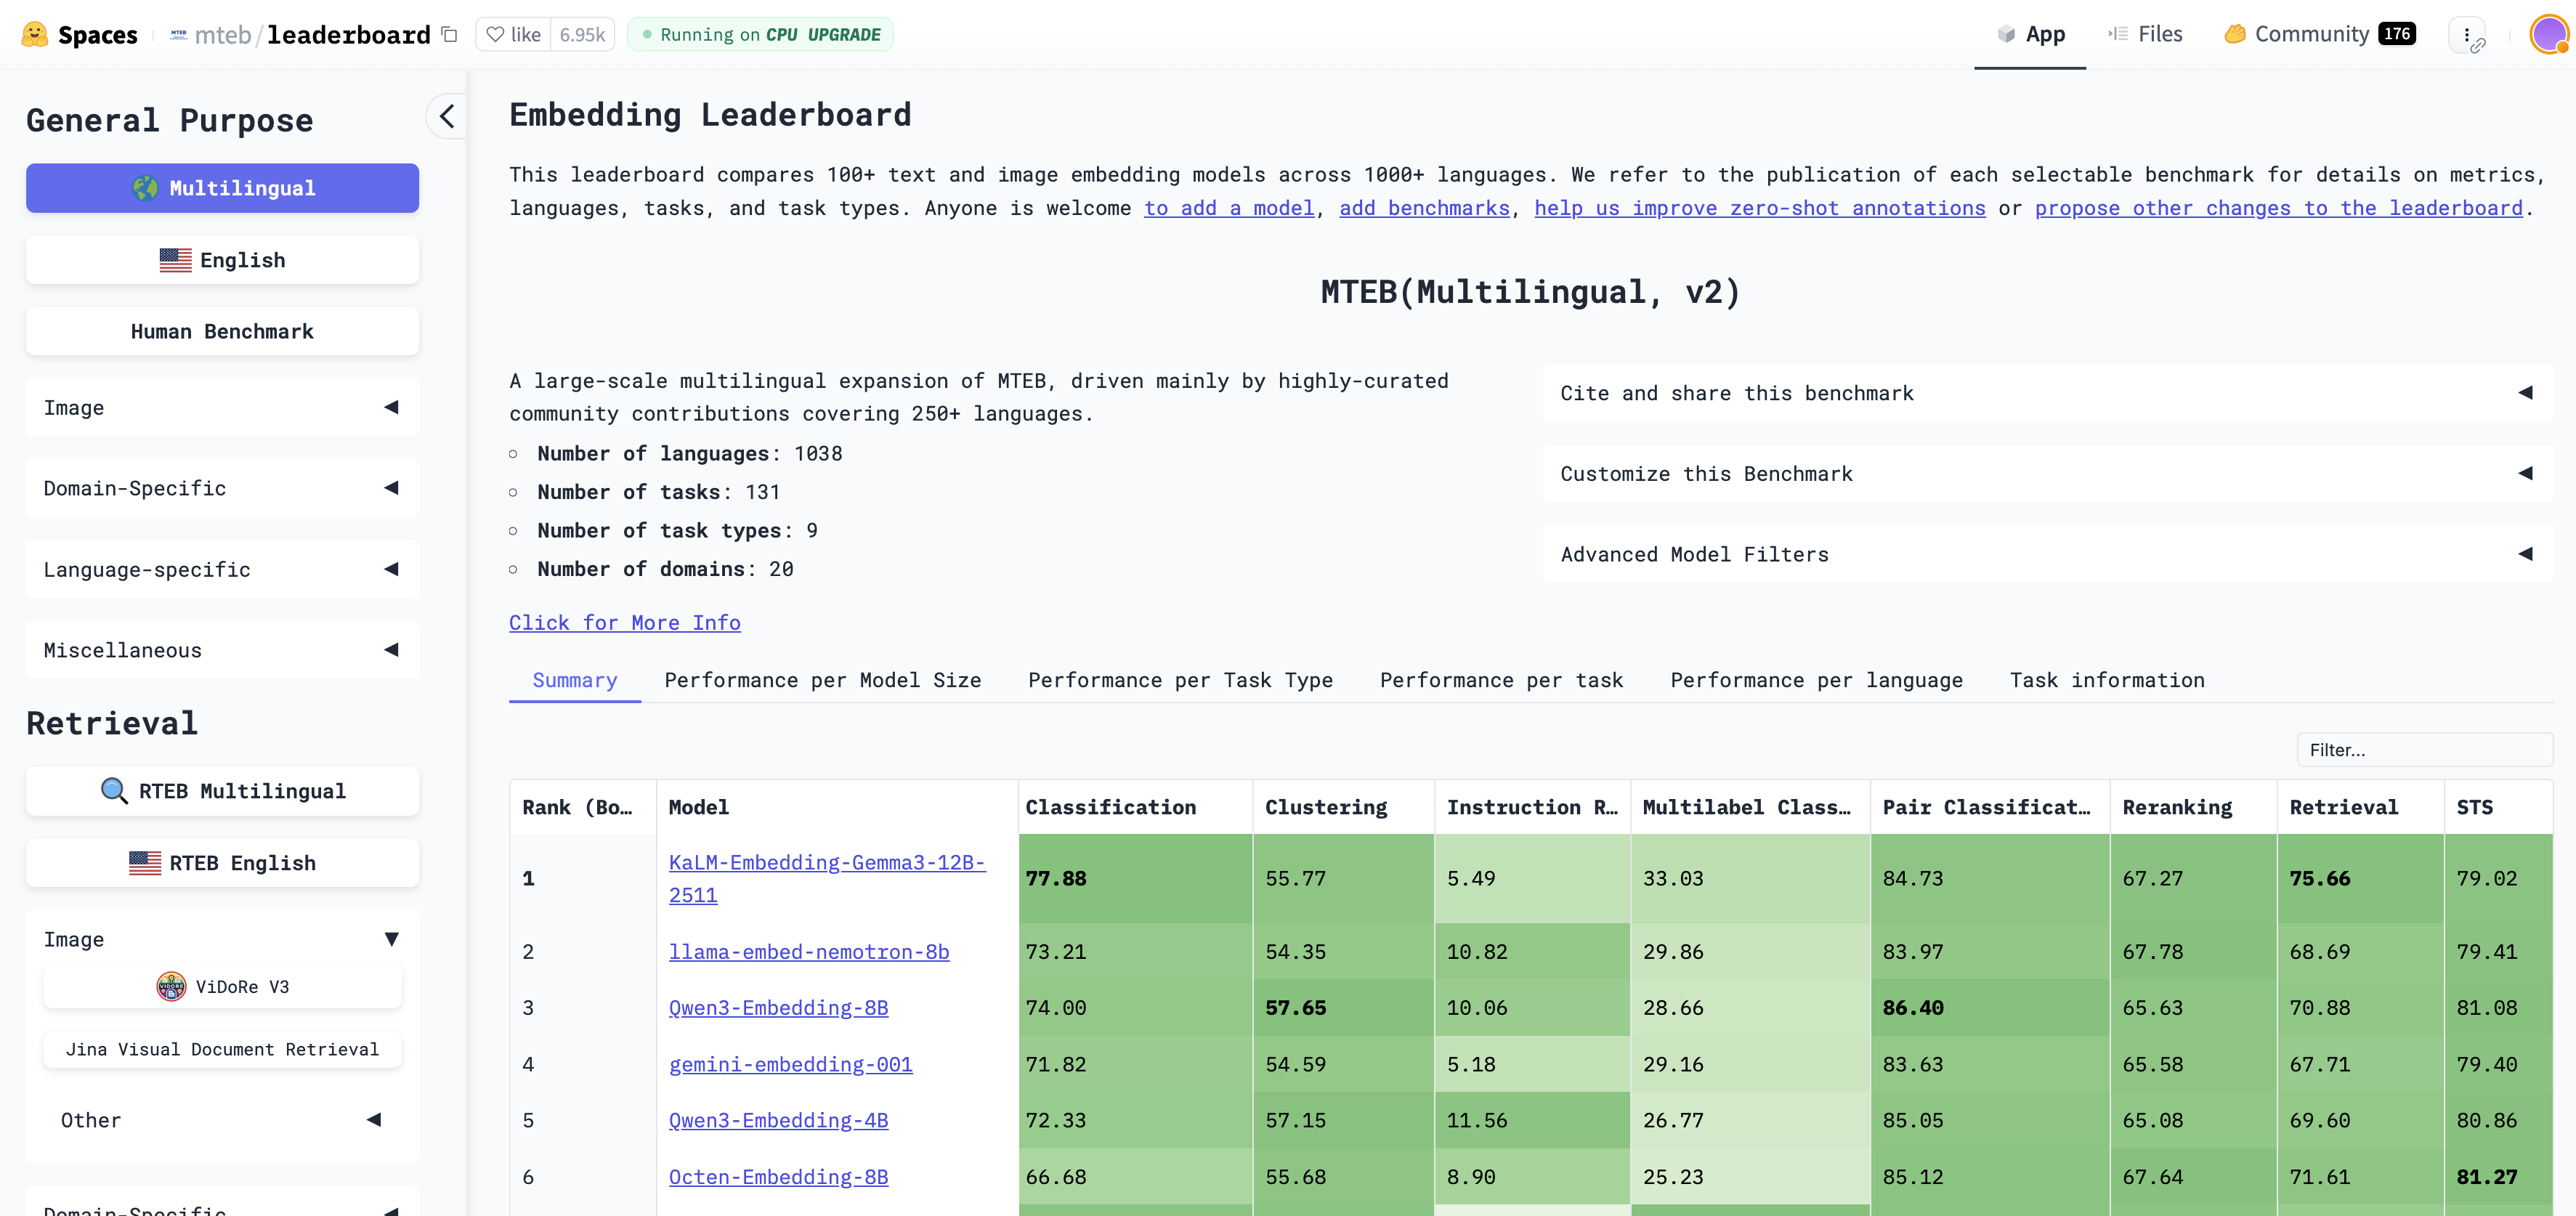
\includegraphics[width=0.75\textwidth,keepaspectratio]{figure/mteb_leaderboard}\\
    \citebutton{Source: MTEB Leaderboard}{https://huggingface.co/spaces/mteb/leaderboard}
\end{center}

\textbf{Practical Implication:} MTEB as reference for embedding models.

\end{frame}

% ------------------------------------------------------------------------------

\begin{frame}{Benchmarks (2): BEIR}

\vfill

\textbf{A diverse information retrieval benchmark:} \citebutton{Thakur et al. (2021) \cite{beir}}{https://datasets-benchmarks-proceedings.neurips.cc/paper/2021/hash/65b9eea6e1cc6bb9f0cd2a47751a186f-Abstract-round2.html}

\begin{itemize}
    \item 18 diverse retrieval datasets
    \item Tests \textbf{zero-shot generalization} across domains
    \item Includes: MS MARCO, Natural Questions, TREC-COVID,etc.
\end{itemize}

\vspace{1em}

\textbf{Why BEIR matters:}
\begin{itemize}
    \item Models often overfit to MS MARCO
    \item BEIR reveals better robustness
    \item Key finding: BM25 often competitive on out-of-domain data
\end{itemize}

\vspace{1em}

\textbf{Smaller version (for limited compute resources):} \citebutton{Nano-BEIR}{https://huggingface.co/blog/sionic-ai/eval-sionic-nano-beir}

\vfill

\end{frame}

% ------------------------------------------------------------------------------

\begin{frame}{Question Types: Single- vs.\ Multi-Hop}

\vfill

\textbf{Single-hop question:} The answer is contained in \textit{one} document.

\begin{tcolorbox}[
    colback=green!6, colframe=green!50!black,
    boxrule=0.8pt, arc=3pt,
    left=6pt, right=6pt, top=4pt, bottom=4pt,
    title={\small\textbf{Example}}, fonttitle=\small
]
{\small \textit{``What is the capital of France?''} $\;\rightarrow\;$ one document suffices}
\end{tcolorbox}

\vspace{.5em}

\textbf{Multi-hop question:} The answer requires \textit{chaining} facts across multiple documents.

\begin{tcolorbox}[
    colback=orange!6, colframe=orange!70!black,
    boxrule=0.8pt, arc=3pt,
    left=6pt, right=6pt, top=4pt, bottom=4pt,
    title={\small\textbf{Example}}, fonttitle=\small
]
\textit{``Where was the director of Oppenheimer born?''}\\[2pt]
{\scriptsize $\rightarrow$ Doc 1: \textit{Nolan directed Oppenheimer}
$\;\xrightarrow{\text{bridges to}}\;$
Doc 2: \textit{Nolan was born in London}}
\end{tcolorbox}

\vspace{.5em}

\textbf{Why does this matter for RAG?}
\begin{itemize}
    \item One-Step-Retrieval handles single-hop questions well
    \item Multi-hop questions \textit{cannot} be answered in a single step\\
    $\rightarrow$ Unclear what to look for in hop 2 before seeing hop 1
\end{itemize}

\vfill

\end{frame}

% ------------------------------------------------------------------------------

\begin{frame}{Multi-Hop Questions: Types}

\vfill

\textbf{Types of multi-hop reasoning:}

\vspace{0.3em}

\begin{itemize}
    \item \textbf{Bridge:} Answer to sub-question 1 is the \textit{entity} to look up next\\
          {\small\textit{``What country is the birthplace of the inventor of the telephone?''}}
    \vspace{0.3em}
    \item \textbf{Intersection:} Answer must satisfy two independent conditions\\
          {\small\textit{``Name a Nolan film starring Cillian Murphy''}}
    \vspace{0.3em}
    \item \textbf{Comparison:} Retrieve facts about two entities, then compare\\
          {\small\textit{``Who is older, Einstein or Bohr?''}}
\end{itemize}

\vspace{1em}

\textbf{Key challenge:} Errors compound -- a wrong first-hop document can easily derail subsequent hops.

\vfill

\end{frame}

% ------------------------------------------------------------------------------
\begin{frame}{Single-Hop vs.\ Multi-Hop: Strategies (1)}

\vfill

\textbf{Single-hop:} One retrieval step is sufficient to answer the question.

\begin{center}
\resizebox{\textwidth}{!}{%
\begin{tikzpicture}[
    node distance=0.5cm,
    box/.style={rectangle, draw=black, thick, minimum height=0.65cm, font=\small, align=center},
    data/.style={rectangle, rounded corners, fill=blue!10, minimum height=0.55cm, font=\small},
    arrow/.style={->, thick, >=stealth}
]
    \node[data] (q1) {``Who wrote \textit{Hamlet}?''};
    \node[box, fill=green!20, right=0.7cm of q1] (r1) {Retriever};
    \node[data, right=0.7cm of r1] (d1) {Doc: Shakespeare};
    \node[box, fill=purple!20, right=0.7cm of d1] (g1) {Generator};
    \node[data, right=0.7cm of g1] (a1) {``Shakespeare''};
    \draw[arrow] (q1) -- (r1);
    \draw[arrow] (r1) -- (d1);
    \draw[arrow] (d1) -- (g1);
    \draw[arrow] (g1) -- (a1);
\end{tikzpicture}
}
\end{center}

\vfill

\textbf{Multi-hop:} The answer requires chaining evidence across multiple documents.

\begin{center}
\resizebox{\textwidth}{!}{%
\begin{tikzpicture}[
    node distance=0.4cm,
    box/.style={rectangle, draw=black, thick, minimum height=0.65cm, font=\small, align=center},
    data/.style={rectangle, rounded corners, fill=blue!10, minimum height=0.55cm, font=\small, align=center},
    arrow/.style={->, thick, >=stealth}
]
    \node[data] (q2) {``Where was the director of\\[-2pt]\textit{Oppenheimer} born?''};
    \node[box, fill=green!20, right=0.5cm of q2] (r2a) {Retriever};
    \node[data, right=0.4cm of r2a, align=center] (d2a) {Doc: Nolan\\directed it};
    \node[box, fill=green!20, right=0.4cm of d2a] (r2b) {Retriever};
    \node[data, right=0.4cm of r2b] (d2b) {Doc: Nolan\\born in London};
    \node[box, fill=purple!20, right=0.4cm of d2b] (g2) {Generator};
    \node[data, right=0.4cm of g2] (a2) {``London''};
    \draw[arrow] (q2) -- (r2a);
    \draw[arrow] (r2a) -- (d2a);
    \draw[arrow] (d2a) -- (r2b);
    \draw[arrow] (r2b) -- (d2b);
    \draw[arrow] (d2b) -- (g2);
    \draw[arrow] (g2) -- (a2);
\end{tikzpicture}
}
\end{center}

\vfill

\end{frame}

% ------------------------------------------------------------------------------

\begin{frame}{Single-Hop vs.\ Multi-Hop: Strategies (2)}

\vfill

\begin{center}
\small
\begin{tabular}{lll}
\toprule
& \textbf{Single-hop} & \textbf{Multi-hop} \\
\midrule
Retrieval steps & 1 & 2+ (iterative) \\
Query & Fixed & Updated after each hop \\
Complexity & Low & High \\
Failure modes & Miss + wrong doc & Error propagation \\
\midrule
Example dataset & Natural Questions & HotpotQA \citebutton{Yang et al. (2018) \cite{yang-etal-2018-hotpotqa}}{https://aclanthology.org/D18-1259/} \\
\bottomrule
\end{tabular}
\end{center}

\vspace{1em}

\textbf{Multi-hop strategies:}
\begin{itemize}
    \item \textbf{Iterative:} Use partial answers to reformulate the query for the next hop
    \item \textbf{Query decomposition:} Break complex question into sub-questions
    \item \textbf{Interleave Chain-of-thought \& retrieval} \citebutton{Trivedi et al. (2023) \cite{trivedi-etal-2023-interleaving}}{https://aclanthology.org/2023.acl-long.557/}
\end{itemize}

\vfill

\end{frame}

% ==============================================================================
% GENERATION EVALUATION
% ==============================================================================

\section{Evaluation (Generator)}

\begin{frame}{Grounding and Source Attribution}

\vfill

\textbf{Overview:}

\vspace{1em}

\footnotesize
\begin{tabular}{p{2.7cm}p{4.2cm}p{3cm}}
\toprule
\textbf{Stage} & \textbf{Approach} & \textbf{Key Methods} \\
\midrule
\textbf{During Generation} & Train/prompt LLM to cite during generating: ``According to [1], ...'' &
\citebutton{Nakano et al. (2022) \cite{nakano2022webgptbrowserassistedquestionansweringhuman}}{https://arxiv.org/abs/2112.09332}
\citebutton{Menick et al. (2022) \cite{menick2022teachinglanguagemodelssupport}}{https://arxiv.org/abs/2203.11147} \\
\addlinespace
\textbf{Reasoning, then generate} & First reason about sources and plan answer, then generate grounded text &
\citebutton{Slobodkin et al. (2024) \cite{slobodkin-etal-2024-attribute}}{https://aclanthology.org/2024.acl-long.182/} \\
\addlinespace
\textbf{Post-hoc Attribution} & Generate first, then retrieve and fact-check each claim and add or fix citations &
\citebutton{Gao et al. (2023) \cite{gao-etal-2023-rarr}}{https://aclanthology.org/2023.acl-long.910/} \\
\bottomrule
\end{tabular}
\normalsize

\vfill

\end{frame}

% ------------------------------------------------------------------------------

\begin{frame}{Prompt Design}

\vfill

\textbf{How retrieved documents reach the generator matters:}

\vspace{0.5em}

\begin{enumerate}
    \item \textbf{Concatenation (standard):}\\
          \texttt{Context: [doc1] [doc2] \ldots [docK]\\Question: \{q\}\\Answer:}
    \vspace{0.4em}
    \item \textbf{Fusion-in-Decoder (FiD)} \citebutton{Izacard \& Grave (2021) \cite{izacard-grave-2021-leveraging}}{https://aclanthology.org/2021.eacl-main.74/}\\
          Encode each (question, passage) pair \textit{separately} with the encoder, then fuse in decoder\\
          $\rightarrow$ Scales to many passages without quadratic attention cost
    \vspace{0.4em}
    \item \textbf{Iterative design:}\\
          Generate intermediate reasoning steps; each step can trigger a new retrieval\\
          $\rightarrow$ cf. \textit{Multi-hop RAG problems}
\end{enumerate}

\vfill

\textbf{Practical recommendation:}\\ Fewer, higher-quality passages often beat many noisy ones.

\vfill

\end{frame}

% ------------------------------------------------------------------------------

\begin{frame}{Faithfulness \& Hallucination Control}

\vspace{1em}

\ques How can we assure that generators do not simply ignore retrieved evidence and fall back on their parametric memory?

\vspace{1em}

\textbf{Approaches to improve faithfulness:}

\vspace{1em}

\begin{itemize}
    \item \textbf{Citation-aware training / prompting:} Ask the model to quote passages inline (e.g.\ WebGPT, GopherCite)
    \item \textbf{Self-RAG} \citebutton{Asai et al. (2024) \cite{asai2024self}}{https://proceedings.iclr.cc/paper_files/paper/2024/file/25f7be9694d7b32d5cc670927b8091e1-Paper-Conference.pdf}\\
          Model learns to decide \textit{when} to retrieve and inserts \textit{reflection tokens} (\texttt{[Retrieve]}, \texttt{[IsRel]}, \texttt{[IsSup]}, \texttt{[IsUse]}) to self-critique its output
			\end{itemize}		
					
\vfill

\end{frame}

% ------------------------------------------------------------------------------

\begin{frame}{Faithfulness \& Hallucination Control}

\vspace{1em}

\ques How can we assure that generators do not simply ignore retrieved evidence and fall back on their parametric memory?

\vspace{1em}

\textbf{Approaches to improve faithfulness:}

\vspace{1em}

\begin{itemize}
    \item \textbf{Constraint decoding:} Force the model to generate tokens that appear in evidence
    \item \textbf{Separate verifier:} A second model checks each claim against retrieved passages
\end{itemize}

\vspace{1em}

\textbf{Key message:} Retrieval quality sets a ceiling; faithfulness techniques help the generator get close to it.

\vfill

\end{frame}

% ------------------------------------------------------------------------------

\begin{frame}{Evaluating RAG Generation}

\vfill

\textbf{Example of generation metrics (there exist many more):}

\vspace{1em}

\small
\begin{tabular}{lll}
\toprule
\textbf{Metric} & \textbf{Measures} & \textbf{How} \\
\midrule
Exact Match (EM) & Correctness & Answer = gold exactly? \\
BERTScore & Semantic similarity & Similarity of answer to gold \\
Faithfulness & Grounding & Is answer supported by docs? \\
\bottomrule
\end{tabular}
\normalsize

\vspace{1em}

\textbf{Practical recommendation:}\\ $\to$ Evaluate components separately to diagnose failures

\vspace{1em}

\textbf{Complete Evaluation Frameworks:} 
	\begin{itemize}
		\item ARES \citebutton{Saad-Falcon et al. (2024) \cite{saad-falcon-etal-2024-ares}}{https://aclanthology.org/2024.naacl-long.20/}     
		\item RAGAs \citebutton{Es et al. (2024) \cite{es-etal-2024-ragas}}{https://aclanthology.org/2024.eacl-demo.16/}  
	\end{itemize}
				
\vfill

\end{frame}

% ==============================================================================
% PART 8: DISCUSSION & SUMMARY (4 slides)
% ==============================================================================

\section{Practical Considerations}

\begin{frame}{Practical Retrieval Pipeline}

\vfill

\begin{center}
\begin{tikzpicture}[
    node distance=0.3cm,
    box/.style={rectangle, draw=black, thick, minimum height=0.5cm, font=\scriptsize},
    data/.style={rectangle, rounded corners, fill=blue!10, minimum height=0.4cm, font=\scriptsize},
    arrow/.style={->, thick, >=stealth}
]
    % Query
    \node[data] (query) {Query};

    % BM25 branch
    \node[box, fill=yellow!30, right=0.6cm of query, yshift=0.4cm] (bm25) {BM25};
    \node[data, right=0.4cm of bm25] (bm25out) {top-100};

    % Dense branch
    \node[box, fill=green!30, right=0.6cm of query, yshift=-0.4cm] (dense) {Dense};
    \node[data, right=0.4cm of dense] (denseout) {top-100};

    % Fusion
    \node[box, fill=orange!30, right=0.8cm of bm25out, yshift=-0.4cm] (rrf) {RRF};
    \node[data, right=0.4cm of rrf] (top100) {top-100};

    % Reranker
    \node[box, fill=purple!30, right=0.4cm of top100] (rerank) {Reranker};
    \node[data, right=0.4cm of rerank] (top10) {top-10};

    % Arrows
    \draw[arrow] (query) |- (bm25);
    \draw[arrow] (query) |- (dense);
    \draw[arrow] (bm25) -- (bm25out);
    \draw[arrow] (dense) -- (denseout);
    \draw[arrow] (bm25out) -- (rrf);
    \draw[arrow] (denseout) -- (rrf);
    \draw[arrow] (rrf) -- (top100);
    \draw[arrow] (top100) -- (rerank);
    \draw[arrow] (rerank) -- (top10);
\end{tikzpicture}
\end{center}

\vfill

\textbf{Reciprocal Rank Fusion:} Document rank aggregation algorithm (based on multiple ranking lists, create unified ranking order)

\vfill

\textbf{Why hybrid (often) wins:}
\begin{itemize}
    \item BM25 catches exact matches 
    \item Dense embeddings catch semantic matches
    \item \textbf{Complementary failure modes} $\rightarrow$ recall improvement
\end{itemize}

\vfill

\end{frame}

% ------------------------------------------------------------------------------

\begin{frame}{Practical Recommendations}

\vfill

\textbf{1. Understand your data:}
\begin{itemize}
    \item What are typical queries? What is your user interested in?
    \item Does the LLM have domain knowledge?
\end{itemize}

\vspace{1em}

\textbf{2. Start simple, iterate:} Many people start with building complex agents.
\begin{enumerate}
    \item BM25 + basic chunking (baseline)
    \item Add hybrid retrieval and reranking
    \item Then add query improvement or agentic behavior. This needs careful design for dedicated datasets
\end{enumerate}

\vspace{1em}

\textbf{3. Monitor:} Evaluate each stage individually

\vfill

\end{frame}


% ------------------------------------------------------------------------------

\section{Case Study}

\begin{frame}{Example: Lost in the Middle (Setup)}

\vfill

\ques Do long-context LLMs use information \textit{uniformly} across positions?
\citebutton{Liu et al. (2024) \cite{liu-etal-2024-lost}}{https://aclanthology.org/2024.tacl-1.9/}

\vspace{1em}

\begin{itemize}
	\item \textit{Experimental Lost in the Middle} (LiM) design:
		\begin{itemize}
		\item Insert one relevant document at varying positions within a long context
		\item Surround it with distractor documents of similar form
		\item Measure answer accuracy as a function of the relevant document's position
		\end{itemize}
	\item Tasks: Multi-document QA and key-value retrieval
	\item This directly probes positional bias in practical long-context usage
\end{itemize}

\vfill

\end{frame}

% ------------------------------------------------------------------------------

\begin{frame}{Example: Lost in the Middle (Main Finding)}

\vspace{1em}

Consistent pattern across models: \textbf{U-shaped performance curve}

\vspace{1em}

\begin{center}
    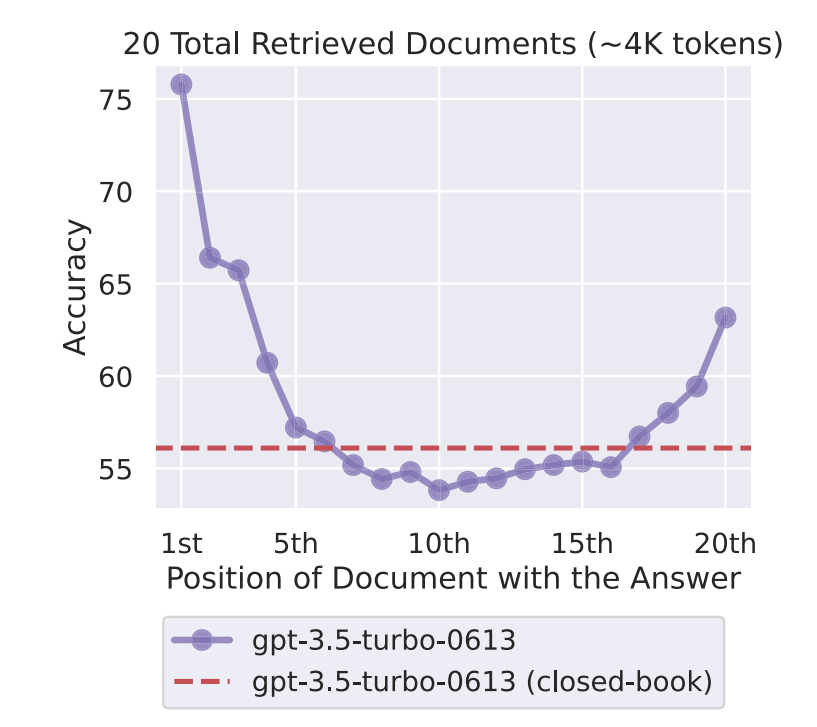
\includegraphics[width=0.6\textwidth,keepaspectratio]{figure/lim}\\
		\citebutton{Source: \cite{liu-etal-2024-lost}}{https://aclanthology.org/2024.tacl-1.9/}
\end{center}


\vfill

\end{frame}

% ------------------------------------------------------------------------------

\begin{frame}{Example: Lost in the Middle (Main Finding)}

\vspace{1em}

Consistent pattern across models: \textbf{U-shaped performance curve}

\vspace{2em}

\begin{itemize}
    \item \textbf{Primacy effect:} Evidence at the \textit{beginning} $\rightarrow$ highest accuracy
    \item \textbf{Recency effect:} Evidence at the \textit{end} $\rightarrow$ second-best accuracy
    \item \textbf{Middle degradation:} Accuracy drops substantially when evidence is buried in the middle
    \item Effect is pronounced even in models with \textbf{32k+ context windows}
    \item[$\Rightarrow$] Larger context window does \textit{not} imply uniform access to all positions
\end{itemize}

\vfill

\end{frame}

% ------------------------------------------------------------------------------

\begin{frame}{Example: Lost in the Middle (Main Finding)}

\vspace{1em}

\textbf{Practical implications for RAG:}

\vspace{2em}

\begin{itemize}
    \item \textbf{Rerank before prompt construction:} Put the most relevant chunks first (or last)
    \item \textbf{Limit the number of passages:} Fewer, better passages beat many mediocre ones
    \item \textbf{Don't (always) assume "more context = better"}
\end{itemize}

\vspace{1em}

\begin{center}
	\warning This behaviour has changed/might change with newer models \warning
\end{center}

\vfill

\end{frame}

% ------------------------------------------------------------------------------

\begin{frame}{Lost in the Middle: Why Does This Happen?}

\vfill

\textbf{Hypothesis 1 -- Attention sink / primacy bias:}
\begin{itemize}
    \item Autoregressive LLMs pay disproportionate attention to early tokens (BOS effect)
    \item Empirically confirmed: attention weights decay toward the middle
\end{itemize}

\vfill

\textbf{Hypothesis 2 -- Training data bias:}
\begin{itemize}
    \item Instruction-tuning data typically has the answer near the beginning or end of provided context $\to$ Model learns a positional shortcut
\end{itemize}

\vfill

\end{frame}

% ------------------------------------------------------------------------------

\begin{frame}{Lost in the Middle: Why Does This Happen?}

\vfill
\textbf{Connections to retrieval:}
\begin{center}
\small
\begin{tabular}{ll}
\toprule
\textbf{Problem} & \textbf{Mitigation} \\
\midrule
Evidence buried in middle & Reranker-ordered prompts \\
Too many passages & Top-$k$ truncation ($k \leq 5$--10) \\
Position-agnostic eval & Shuffle eval (test robustness) \\
\bottomrule
\end{tabular}
\end{center}

\vfill

\textbf{Open questions:} 
	\begin{itemize}
		\item Does instruction tuning on position-diverse data help? \citebutton{Liu et al. (2024) \cite{liu-etal-2024-lost}}{https://aclanthology.org/2024.tacl-1.9/}
		\item What is the role of positional encoding? \citebutton{Zehle \& Aßenmacher (2026) \cite{zehle-assenmacher-2026-calibration}}{https://aclanthology.org/2026.findings-eacl.120/}
	\end{itemize}

\vfill

\end{frame}

% ==============================================================================

\begin{frame}[allowframebreaks,noframenumbering,plain]{References}
        \tiny
        \bibliographystyle{plain} %apalike
        \bibliography{refs-rag}
\end{frame}

\endlecture
\end{document}
